%\documentclass[journal,twocolumn]{IEEEtran}
\documentclass[10pt,conference]{IEEEtran}
% ── Core packages ─────────────────────────────────────────────────────
\usepackage[T1]{fontenc}
\usepackage{amsmath,amssymb,amsfonts}
\usepackage{algorithmic}
\usepackage{algorithm}
\usepackage{graphicx}
\usepackage{textcomp}
\usepackage{xcolor}
\usepackage{booktabs}
\usepackage{cite}
\usepackage{multirow}
\usepackage{array}
\usepackage{bm}
\usepackage{balance}
\usepackage[caption=false,font=footnotesize]{subfig}
%\usepackage{url}

\graphicspath{{./}{../../outputs_joint_ao/ieee_plots/}}


% ── Math shortcuts ────────────────────────────────────────────────────
\newcommand{\vect}[1]{\mathbf{#1}}
\newcommand{\mat}[1]{\mathbf{#1}}
\newcommand{\E}{\mathbb{E}}
\newcommand{\R}{\mathbb{R}}
\newcommand{\C}{\mathbb{C}}
\DeclareMathOperator{\diag}{diag}
\DeclareMathOperator{\Tr}{Tr}
\DeclareMathOperator*{\argmax}{arg\,max}
\DeclareMathOperator*{\argmin}{arg\,min}
\newcommand{\dBm}{\,\text{dBm}}
\newcommand{\dB}{\,\text{dB}}
\newcommand{\GHz}{\,\text{GHz}}

\begin{document}

% ══════════════════════════════════════════════════════════════════════
% TITLE
% ══════════════════════════════════════════════════════════════════════

\title{IRS-Assisted Learning-Based Anti-Jamming for Wideband THz Communications}
%\title{IRS-Assisted Anti-Jamming for Wideband THz Communications: A Reinforcement Learning and Alternating Optimization Framework}

\author{Anuprabh Singh, Sourabh Solanki, Ugrasen Singh
\thanks{Anuprabh Singh and Sourabh Solanki are with the Department of Electronics and Communication Engineering, National Institute of Technology, Warangal 506004, India (e-mail: anuprabh@student.nitw.ac.in).}}

\maketitle

% ══════════════════════════════════════════════════════════════════════
% ABSTRACT
% ══════════════════════════════════════════════════════════════════════

\begin{abstract}
Wideband terahertz (THz) communication systems are highly vulnerable to intelligent jamming due to frequency-selective propagation, beam squint, and highly directional transmissions. This paper proposes an intelligent reflecting surface (IRS)-assisted anti-jamming framework for wideband THz OFDM systems that jointly optimizes transmit power allocation, IRS phase configuration, and hybrid beamforming. The resulting non-convex problem is solved by a three-block framework in which a fuzzy Win-or-Learn-Fast Policy Hill-Climbing algorithm adapts power allocation against a smart jammer, while the IRS configuration and beamformer are updated through low-complexity per-block surrogate objectives with closed-form solutions and frequency-dependent sub-array control that compensates beam squint. The proposed method achieves a system rate of 11.87 bits/s/Hz and a signal-to-interference-plus-noise ratio (SINR) protection level of 81.6\% (fraction of user--subcarrier pairs meeting the $\gamma_{\min}=5$\,dB target), improving on the strongest reinforcement-learning or deterministic baseline per metric by 44\% in throughput and 66\% in protection.

\end{abstract}

\begin{IEEEkeywords}
Terahertz communications, intelligent reflecting surfaces, anti-jamming communications, reinforcement learning, hybrid beamforming, beam squint, physical layer security.
\end{IEEEkeywords}
% ══════════════════════════════════════════════════════════════════════
\section{Introduction}
\label{sec:intro}
\IEEEPARstart{T}{erahertz} (THz) communication is a promising enabler of sixth-generation (6G) networks owing to its ultra-wide bandwidth, but its propagation suffers from severe path loss, molecular absorption, and sparse scattering, necessitating highly directional beamforming with large antenna arrays \cite{su2023wideband,yan2023beamforming}. Directionality, however, does not eliminate security vulnerabilities: intentional jamming remains a major threat. Traditional anti-jamming techniques such as frequency hopping and adaptive transmission are effective in conventional systems \cite{hanawal2016joint,xu2018jamming}, but the frequency-selective, absorption-dominated THz channel complicates their direct application \cite{akyildiz2022thz}.

Recently, intelligent reflecting surfaces (IRSs) have attracted considerable attention as a cost-effective means of enhancing coverage, spectral efficiency, and physical-layer security by reshaping the propagation environment through passive phase control \cite{wu2019intelligent,wu2021irs_survey,renzo2020smart}. Combined with reinforcement learning (RL), IRS-assisted anti-jamming can adapt to unknown and time-varying jammer behavior \cite{yang2021irs}.

Despite these advances, important challenges remain. Most existing IRS-assisted anti-jamming studies are narrowband and ignore the frequency selectivity of wideband THz channels \cite{yang2021irs}; beam-squint effects of large bandwidths and arrays are often overlooked despite their severe impact on beamforming gain \cite{su2023wideband,yan2023beamforming}; many RL-based schemes rely on deterministic, predictable policies that intelligent adversaries can exploit; and the joint optimization of power allocation, IRS configuration, and hybrid beamforming under adaptive jamming remains open for wideband THz systems.

The main contributions are as follows:
\begin{itemize}
\item We formulate a joint optimization of transmit power allocation, IRS phase design, and sub-connected hybrid beamforming for IRS-assisted anti-jamming in wideband THz orthogonal frequency-division multiplexing (OFDM) systems, and solve the resulting non-convex problem with a three-block RL and alternating optimization (RL--AO) framework combining learning-based power allocation with low-complexity surrogate updates of the IRS and beamforming variables.

\item We propose a fuzzy Win-or-Learn-Fast Policy Hill-Climbing (F-WoLF-PHC) algorithm that integrates fuzzy state aggregation and mixed-strategy learning to resist policy-exploiting intelligent jammers.

\item We integrate a sub-connected phase-delay-phase (SPDP) IRS beam-squint compensation architecture (adapted from~\cite{su2023wideband}) into the RL--AO framework, extending it with a multi-user AoD candidate search that re-optimizes the wideband IRS configuration jointly with the RL agent's instantaneous power allocation.

\item Extensive simulations demonstrate significant throughput and signal-to-interference-plus-noise ratio (SINR) protection gains over RL and deterministic baselines.
\end{itemize}
%\emph{Notation:} Bold lower/uppercase denotes vectors/matrices; $(\cdot)^H$, $|\cdot|$, $\|\cdot\|$, $\diag(\cdot)$, and $\mathbf{1}\{\cdot\}$ have standard meanings.
\section{System Model and Problem Formulation}
\label{sec:system}
\subsection{Network Architecture}
We consider a downlink wideband THz OFDM system comprising a base station (BS) with $N$ antennas and $N_{\mathrm{RF}}$ RF chains in a sub-connected hybrid analog-digital architecture, an $M$-element planar IRS, $K$ single-antenna users, and an adaptive jammer with $N_J$ antennas ($N_J=2$ in our evaluation). The system operates at carrier frequency $f_c$ with bandwidth $B$ divided into $M_{\mathrm{sc}}$ OFDM subcarriers. Since the jammer interferes with each user directly, the IRS does not null the jamming signal; instead, it improves anti-jamming resilience by strengthening the desired effective channel, thereby increasing the SINR margin under jamming.

Let $\mathbf{G}[m] \in \mathbb{C}^{M \times N}$ denote the BS-to-IRS channel on subcarrier $m$, $\mathbf{h}_{ru,k}[m] \in \mathbb{C}^{M}$ the IRS-to-user-$k$ channel, and $\mathbf{h}_{bu,k}[m] \in \mathbb{C}^{N}$ the direct BS-to-user-$k$ channel. The jammer-to-user-$k$ channel is denoted by $\mathbf{h}_{J,k} \in \mathbb{C}^{N_J}$ and is modeled as frequency-flat. Further, the IRS reflection matrix on subcarrier $m$ is defined as
%\begin{equation}
$\boldsymbol{\Phi}[m] = \mathrm{diag}\left(e^{j\theta_1[m]}, \ldots, e^{j\theta_M[m]}\right)$,
%\end{equation}
where $\theta_i[m]$ represents the phase shift of the $i$-th reflecting element. The effective channel between the BS and user $k$ is expressed as
%\begin{equation}
$\mathbf{h}_{\mathrm{eff},k}[m] =
\mathbf{G}^H[m]\boldsymbol{\Phi}^H[m]\mathbf{h}_{ru,k}[m] + \mathbf{h}_{bu,k}[m].$
%\end{equation}
We assume the BS has perfect instantaneous channel state information (CSI) of $\mathbf{G}[m]$, $\mathbf{h}_{ru,k}[m]$, and $\mathbf{h}_{bu,k}[m]$ for IRS and beamformer design, a common idealization that isolates the achievable RL--AO performance from channel-estimation error. The jammer's channel and strategy remain unknown to the BS and are inferred only indirectly through SINR feedback and observed action predictability (Sec.~\ref{sec:rl}-F); $\mathbf{h}_{J,k}$ enters the SINR \eqref{eq:sinr} only for performance evaluation by the simulated environment and is never used by the transmitter-side optimization. Imperfect BS-side CSI is left to future work.

\subsection{THz Channel Model}

THz channels exhibit strong frequency selectivity due to molecular absorption and beam-squint effects. The BS-IRS channel on subcarrier $m$ is modeled using a geometry-based Saleh--Valenzuela representation~\cite{su2023wideband}:
\begin{equation}
\mat{G}[m] = \sqrt{\frac{N M}{L_{\text{path}}}} \sum_{\ell=1}^{L_{\text{path}}} \alpha_\ell(f_m)\, \vect{a}_{\text{IRS}}(\phi_\ell, f_m) \vect{a}_{\text{BS}}^H(\psi_\ell, f_m)
\label{eq:thz_channel}
\end{equation}
where $L_{\text{path}}$ is the number of propagation paths, $\alpha_\ell(f_m)$ is the complex path gain at subcarrier frequency $f_m = f_c + (m - M_{\text{sc}}/2)\Delta f$ with subcarrier spacing $\Delta f = B/M_{\text{sc}}$, and $\vect{a}_{\text{IRS}}$, $\vect{a}_{\text{BS}}$ are frequency-dependent array steering vectors. The frequency dependence of the steering vectors is the root cause of beam squint, as the spatial angle-of-arrival/departure at which constructive interference occurs shifts with frequency.

%\subsection{Path Loss and Molecular Absorption}

The THz path loss at frequency $f$ and distance $d$ is
\begin{equation}
\text{PL}(f, d) = \left(\frac{4\pi f d}{c}\right)^2 e^{\kappa_{\text{abs}}(f) d}
\label{eq:pathloss}
\end{equation}
where $c$ is the speed of light and $\kappa_{\text{abs}}(f)$ is the molecular absorption coefficient; $\text{PL}(f,d)$ is a linear (power-scale) factor. The complex path gain in \eqref{eq:thz_channel} subsumes this attenuation, i.e., $\alpha_\ell(f_m) = \text{PL}^{-1/2}(f_m, d_\ell)\, e^{-j2\pi f_m d_\ell / c}$, so path loss and absorption enter the model exactly once. Unlike microwave channels, $\kappa_{\text{abs}}(f)$ varies within the 10\,GHz bandwidth, introducing per-subcarrier attenuation diversity. In the LoS-dominant THz regime adopted for evaluation, \eqref{eq:thz_channel} is used with $L_{\text{path}}=1$.

\subsection{SPDP-IRS Architecture for Beam-Squint Compensation}

To maintain beam alignment across the wideband THz spectrum, the IRS employs the sub-connected phase-delay-phase (SPDP) architecture proposed in~\cite{su2023wideband}: the $M$ reflecting elements are partitioned into $Q = 64$ sub-arrays, each element retains its own phase shifter, and each sub-array is additionally driven by a shared true-time-delay (TTD) module that realizes a frequency-proportional phase across the band. The reflection phase of element $i$ in sub-array $q$ is
\begin{equation}
\theta_{q,i}[m] = \theta_{q,i}^{\text{base}} + 2\pi f_m \tau_q
\label{eq:spdp}
\end{equation}
where $\theta_{q,i}^{\text{base}}$ is the base phase and $\tau_q$ is the TTD delay for sub-array $q$. This keeps the beam direction consistent across subcarriers and avoids edge-subcarrier gain loss. A TTD-assisted IRS is not purely passive in the strict sense: the $Q$ TTD modules are active, though few relative to $M$ ($Q/M=1/4$ here), while the per-element phase shifters remain passive~\cite{su2023wideband}. As in~\cite{su2023wideband}, we assume ideal (lossless) TTDs and continuous phase shifters; quantization and insertion loss are left to future work.

\subsection{Signal Model}

The received signal at user $k$ on subcarrier $m$ is given by
\begin{align}
\begin{split}
y_k[m] &= \mathbf{h}_{\mathrm{eff},k}^H[m]\mathbf{w}_k[m]\sqrt{P_k}s_k + \sum_{i \neq k} \mathbf{h}_{\mathrm{eff},k}^H[m]\mathbf{w}_i[m]\sqrt{P_i}s_i \\ 
&+ \mathbf{h}_{J,k}^H \mathbf{z}_k \sqrt{P_{J,k}} j_k + n_k,  
\end{split}
\end{align}
where $\mathbf{w}_k[m]$ is the hybrid beamforming vector, $P_k$ is the transmit power allocated to user $k$, $s_k$ is the unit-power data symbol ($\E[|s_k|^2]=1$), $P_{J,k}$ and $\mathbf{z}_k \in \mathbb{C}^{N_J}$ denote the jammer power and spatial precoder with $\|\mathbf{z}_k\|=1$, $j_k$ is the unit-power jamming symbol ($\E[|j_k|^2]=1$), and $n_k$ is additive white Gaussian noise with per-subcarrier variance
\begin{equation}
\sigma^2 = k_B T \, \frac{B}{M_{\mathrm{sc}}} \cdot 10^{F_{\mathrm{NF}}/10},
\label{eq:noise}
\end{equation}
where $k_B$ is Boltzmann's constant, $T=290$\,K, $B/M_{\mathrm{sc}}$ is the per-subcarrier bandwidth, and $F_{\mathrm{NF}}=10$\,dB is the receiver noise figure; for $B=10$\,GHz and $M_{\mathrm{sc}}=64$ this yields $\sigma^2 \approx -82$\,dBm per subcarrier.
The SINR of user $k$ on subcarrier $m$ is defined as
\begin{equation}
\mathrm{SINR}_k[m] \!=\!
\frac{P_k |\mathbf{h}_{\mathrm{eff},k}^H[m]\mathbf{w}_k[m]|^2}
{\sum_{i \neq k}\! P_i |\mathbf{h}_{\mathrm{eff},k}^H[m]\mathbf{w}_i[m]|^2
\!+ \!P_{J,k} |\mathbf{h}_{J,k}^H \mathbf{z}_k|^2 \!+\! \sigma^2 }.
\label{eq:sinr}
\end{equation}
The achievable rate of user $k$ is
\begin{equation}
R_k = \frac{1}{M_{\mathrm{sc}}} \sum_{m=1}^{M_{\mathrm{sc}}}
\log_2\left(1 + \mathrm{SINR}_k[m]\right),
\label{eq:rate}
\end{equation}
and the sum rate is $R_{\mathrm{sum}} = \sum_{k=1}^{K} R_k$.
To quantify quality-of-service (QoS) satisfaction under jamming, the SINR protection ratio is defined as
\begin{equation}
\eta_{\mathrm{prot}} =
\frac{1}{K M_{\mathrm{sc}}}
\sum_{k=1}^{K}\sum_{m=1}^{M_{\mathrm{sc}}}
\mathbf{1}\{\mathrm{SINR}_k[m] \geq \gamma_{\min}\},
\label{eq:prot}
\end{equation}
where $\gamma_{\min}$ is the minimum SINR threshold. Throughout the paper, $\gamma_{\min}$ is specified in dB (Table~\ref{tab:params}) and converted to linear scale wherever it is compared against a linear SINR, as in \eqref{eq:prot} and \eqref{eq:qos}.

\subsection{Hybrid Beamforming}
Each RF chain drives a dedicated subset of $N_{\mathrm{per}} = N/N_{\mathrm{RF}}$ antennas through analog phase shifters, yielding a block-diagonal analog precoder. The transmit beamforming vector for user $k$ on subcarrier $m$ is
\begin{equation}
\vect{w}_k[m] = \mat{F}_{\text{RF}} \vect{f}_{BB,k}[m]
\label{eq:hybrid_bf}
\end{equation}
where $\mat{F}_{\text{RF}} \in \C^{N \times N_{\text{RF}}}$ is the frequency-flat analog precoder (block-diagonal, constant-modulus entries) and $\vect{f}_{BB,k}[m] \in \C^{N_{\text{RF}}}$ is the per-subcarrier digital precoder. The digital precoder adopts a max-SINR (Minimum Variance Distortionless Response (MVDR)) design. For user $k$ at subcarrier $m$, the interference-plus-noise covariance is
\begin{equation}
\mat{R}_k[m] = \sigma^2\mat{I} + \sum_{i \neq k}P_i\,\tilde{\vect{h}}_i[m]\tilde{\vect{h}}_i^H[m]
\label{eq:Rk}
\end{equation}
where $\tilde{\vect{h}}_i[m] = \mat{F}_{\text{RF}}^H\vect{h}_{\text{eff},i}[m]$ is the compressed effective channel of user $i$ (any $i \in \{1,\dots,K\}$); $\mat{R}_k[m]$ thus collects transmit-side leakage from the \emph{other} users' channels plus noise, suppressing inter-user leakage at the transmitter rather than modeling receiver-side interference. The MVDR precoder is
\begin{equation}
\vect{f}_{BB,k}[m] = \frac{\mat{R}_k^{-1}[m]\tilde{\vect{h}}_k[m]}{\|\mat{R}_k^{-1}[m]\tilde{\vect{h}}_k[m]\|}.
\label{eq:mvdr}
\end{equation}


\subsection{Joint Optimization Problem}

The objective is to maximize the system sum rate by jointly optimizing transmit power allocation, IRS phase shifts, and hybrid beamforming under QoS and hardware constraints. The optimization problem is formulated as
\begin{subequations}
\begin{align}
\max_{\{P_k\}, \{\boldsymbol{\Phi}[m]\}, \mathbf{F}_{\mathrm{RF}}, \{\mathbf{f}_{\mathrm{BB},k}[m]\}}
& \quad R_{\mathrm{sum}} \label{eq:obj}\\
\text{s.t.} \quad
& \sum_{k=1}^{K} P_k \leq P_{\max},\label{eq:power} \\
& \mathrm{SINR}_k[m] \geq \gamma_{\min}, \ \forall k,m, \label{eq:qos}\\
& |[\boldsymbol{\Phi}[m]]_{i,i}| = 1, \ \forall i,m, \label{eq:unit}\\
& \mathbf{F}_{\mathrm{RF}} \in \mathcal{F}_{\mathrm{RF}}, \label{eq:bc}\\
%& [\mat{F}_{\text{RF}}]_{ij} = 0,\ \forall (i,j) \notin \mathcal{S}_{\text{BC}} \label{eq:bc}\\ 
%& |[\mat{F}_{\text{RF}}]_{ij}| = \tfrac{1}{\sqrt{N_{\text{per}}}},\ \forall (i,j) \in \mathcal{S}_{\text{BC}} \label{eq:cm}\\
& \|\mathbf{F}_{\mathrm{RF}}\mathbf{f}_{\mathrm{BB},k}[m]\|^2 \leq 1, \ \forall k,m,\label{eq:pn}
\end{align}
\end{subequations}
where $\mathcal{F}_{\mathrm{RF}}$ denotes the set of sub-connected constant-modulus analog precoders imposed by the RF hardware architecture.

The per-user, per-subcarrier QoS constraint \eqref{eq:qos} may be infeasible under sufficiently strong jamming, since the jammer term in \eqref{eq:sinr} is outside the BS's control; \eqref{eq:qos} therefore formalizes the design target, and the proposed solver treats it as a soft constraint enforced through the continuous SINR-deficit penalty in the RL reward \eqref{eq:reward}, which degrades gracefully instead of rendering the problem infeasible. The problem is highly non-convex due to the coupling among the variable blocks and the unit-modulus/constant-modulus constraints, and the adaptive jammer's strategy is unknown a priori, making purely deterministic, model-based optimization ineffective.

\section{Proposed RL--AO Anti-Jamming Framework}
\label{sec:rl}

\subsection{RL--AO Problem Decomposition}

The optimization variables in \eqref{eq:obj}--\eqref{eq:pn} are partitioned into three blocks --- transmit power allocation $\{P_k\}$, IRS phase shifts $\{\boldsymbol{\Phi}[m]\}$, and hybrid beamforming variables $\{\mat{F}_{\mathrm{RF}},\vect{f}_{BB,k}[m]\}$ --- with reinforcement learning determining the power-allocation policy and alternating optimization updating the IRS and beamforming variables:
\begin{enumerate}
\item \textbf{Block 1 --- Power allocation (RL):} The RL agent selects an action from $\mathcal{A}$ ($|\mathcal{A}|=42$), the Cartesian product of 7 total-power fractions and 6 per-user allocation modes (Table~\ref{tab:actions}). This block handles the combinatorial, model-free nature of the adversarial environment.
\item \textbf{Block 2 --- IRS phase shifts (surrogate AO):} Given $\{P_k\}$ and $\mat{F}_{\text{RF}}$, the IRS phases are obtained from a per-element closed-form expression that maximizes the aggregate \emph{desired} signal power. This is a tractable surrogate for \eqref{eq:obj}: it deliberately ignores multi-user interference and the jammer term (which are handled by the MVDR digital precoder and the RL power policy, respectively) and is not an exact solution of the coupled SINR objective.
\item \textbf{Block 3 --- Hybrid beamforming:} Given $\{P_k\}$ and $\{\bm{\Phi}[m]\}$, the analog precoder is updated by SVD-based dominant-subspace projection under the constant-modulus constraint, and the digital precoder is re-solved via MVDR~\eqref{eq:mvdr}.
\end{enumerate}

Per-user weights are computed from the current channel/SINR state, normalized to sum to one, and scaled by the chosen power fraction, so every action satisfies \eqref{eq:power} by construction. All SINR-dependent weights use \emph{linear-scale} SINR floored at $\epsilon = 10^{-12}$, keeping the inverse-SINR and deficit modes well defined in deep outage.

At each environment step the RL agent first selects a power-allocation action, after which the IRS phases and beamforming variables are updated via AO for $N_{\mathrm{AO}}=3$ inner iterations, letting the learning module focus on adversarial decision-making while the continuous variables track instantaneous CSI.

\begin{table}[t]
\centering
\caption{Power-Allocation Action Space ($7 \times 6 = 42$ Actions)}
\label{tab:actions}
\begin{tabular}{ll}
\toprule
\multicolumn{2}{l}{Total power fraction $P_{\mathrm{tot}}/P_{\max} \in \{0.20, 0.35, 0.50, 0.65, 0.80, 0.90, 1.00\}$} \\
\midrule
\textbf{Allocation mode} & \textbf{Per-user weight} \\
\midrule
Equal & uniform, $1/K$ each \\
Channel-proportional & $\propto$ channel quality \\
Inverse-channel & $\propto 1/(\text{channel quality})$ \\
SINR-deficit & $\propto \max(0,\gamma_{\min}{-}\text{SINR}_k)$ \\
Water-filling & $\propto \log(1{+}\text{channel quality})$ \\
Max-protection & $\propto 1/\max(\text{SINR}_k, \epsilon)$ (worst-user focus) \\
\bottomrule
\end{tabular}
\end{table}

\subsubsection{Block 2--IRS Phase Optimization via AO}
Given $\{P_k\}$, the IRS phases follow the SPDP design of Sec.~\ref{sec:system}-C~\eqref{eq:spdp}: per-element phases align the BS-to-IRS angle-of-arrival and a reference AoD across each sub-array (the cascade design thus uses both arrival and departure geometry), with the residual frequency-dependent phase compensated by $\tau_q$. Since one reference AoD cannot align the cascaded geometry of all $K$ users, it is re-optimized every $N_{\mathrm{AO}}$ steps over $K+1$ candidates (the per-user AoDs and their centroid), each scored by the \emph{achieved} $R_{\mathrm{sum}}$ under the current $\{P_k\}$ and $\mat{F}_{\text{RF}}$ rather than by geometric alignment alone; whenever the centroid fails to preserve the cascade geometry, an individual user AoD is selected instead.

\subsubsection{Block 3--Analog Precoder Update via SVD}
Since $\mat{F}_{\text{RF}}$ is frequency-flat, the effective channel is aggregated over reference subcarriers as $\overline{\mat{H}} = \sum_{m \in \mathcal{M}_{\text{ref}}} \vect{H}_{\text{eff}}^H[m]$; each sub-array partition $\overline{\mat{H}}_p$ is SVD-decomposed, the analog column updated as $[\mat{F}_{\text{RF}}]_p = \exp(j\angle\vect{u}_p)/\sqrt{N_{\text{per}}}$ (unit-modulus projection), and $\{\vect{f}_{BB,k}[m]\}$ re-solved via MVDR~\eqref{eq:mvdr}.


\subsection{State Representation}

The system state is a compact feature vector
$\mathbf{f} = [f_{\mathrm{pj}}, f_{\mathrm{ch}}, f_{\mathrm{sinr}}] \in [0,1]^3$ capturing jammer activity, channel condition, and SINR quality. All features are computed from dB-scale quantities and normalized by $\text{norm}_{[a,b]}(x) = \text{clip}\!\big((x-a)/(b-a),\,0,\,1\big)$ with THz-calibrated ranges $[a,b]$:
\begin{align}
f_{\mathrm{pj}} &=
\text{norm}_{[0,25]}\!\left(
0.6\,\overline{P_J} + 0.4\,\max_k P_{J,k}
\right), \label{eq:fpj}\\
f_{\mathrm{ch}} &=
0.75\,\text{norm}_{[-160,-60]}\!\left(\overline{g_k}\right) + 0.25\,(1-s_{\mathrm{ch}}), \label{eq:fch}\\
f_{\mathrm{sinr}} &=
\text{norm}_{[-20,30]}\!\left(
0.5\,\overline{\mathrm{SINR}_k} + 0.5\,\min_k \mathrm{SINR}_k
\right), \label{eq:fsinr}
\end{align}
where $\overline{P_J}$ and $P_{J,k}$ are jammer powers in dBm; $g_k = 10\log_{10}\|\mathbf{h}_{\mathrm{eff},k}\|^2$ is the subcarrier-averaged effective channel gain of user $k$ in dB with mean $\overline{g_k}$ over users and normalized (dimensionless) spread $s_{\mathrm{ch}} = \min\!\big(\mathrm{std}_k(g_k)/30,\,1\big)$, so both terms of \eqref{eq:fch} are dimensionless before combination; and $\mathrm{SINR}_k$ in \eqref{eq:fsinr} is the subcarrier-averaged SINR of user $k$ in dB.

For tabular baselines, each feature is uniformly quantized into $B_q=8$ levels ($8^3=512$ discrete states); the proposed WoLF-PHC instead operates on continuous inputs via fuzzy state aggregation, avoiding discretization loss.


\subsection{Fuzzy State Aggregation}

Each feature $x \in [0,1]$ is mapped to three triangular memberships with centers $\{0,0.5,1.0\}$:
\begin{equation}
\mu_i(x) = \frac{\max(0, 1 - |x - c_i|/\Delta)}{\sum_j \max(0, 1 - |x - c_j|/\Delta)}
\label{eq:fuzzy}
\end{equation}
where $\Delta = 0.5$ is the spread parameter. The joint fuzzy membership vector has $3^3 = 27$ components:
\begin{equation}
\psi_\ell(\vect{f}) = \mu_i(f_{\text{pj}}) \cdot \mu_j(f_{\text{ch}}) \cdot \mu_k(f_{\text{sinr}}), \quad \ell = 9i + 3j + k,
\label{eq:fuzzy_joint}
\end{equation}
where $i,j,k \in \{0,1,2\}$ are zero-based indices of the membership centers, so that $\ell \in \{0,\dots,26\}$; this smooths state transitions and improves robustness.

\subsection{Proposed Fuzzy WoLF-PHC Algorithm}

WoLF-PHC~\cite{bowling2002wolf} learns faster when losing and slower when winning. The fuzzy version maintains, for each of the 27 fuzzy rules $\ell$, a Q-table $Q_\ell(s,a)$, a policy $\pi_\ell(a)$, and an average policy $\bar{\pi}_\ell(a)$, where $s$ is the \emph{discrete} state index from the $B_q=8$-level quantization of Sec.~\ref{sec:rl}-B (not the continuous feature vector): each rule keeps its own table over the $8^3$ discrete states, the continuous features enter only through the memberships $\psi_\ell(\vect{f})$, and the policies are indexed by the rule alone.

\subsubsection{Fused Q-Value}
Each observation maps to the pair $\big(s, \bm{\psi}(\vect{f})\big)$; the effective Q-value is the fuzzy-weighted combination
\begin{equation}
\text{FQ}(s, a) = \sum_{\ell=0}^{26}\psi_\ell(\vect{f}) \cdot Q_\ell(s, a).
\label{eq:fused_q}
\end{equation}

\subsubsection{Q-Update}
Following the fuzzy Q-learning convention, every active rule $\ell$ ($\psi_\ell > 0$) is updated toward a common target,
\begin{equation}
Q_\ell(s,a) \leftarrow (1-\alpha)\,Q_\ell(s,a) + \alpha\left[r + \gamma\max_{a'}\text{FQ}(s',a')\right]
\label{eq:q_update}
\end{equation}
where $\gamma = 0.9$ is the discount factor and $\alpha$ is a visit-count-adaptive learning rate shared by all rules at a given step,
\begin{equation}
\alpha = \min\!\left(1,\ \alpha_0\Big(1 + \frac{3}{1+0.1\,n(s,a)}\Big)\right),
\label{eq:alpha_adaptive}
\end{equation}
with base rate $\alpha_0=0.01$ and $n(s,a)$ the visit count of the discrete state--action pair (one counter shared across rules); learning is boosted for rarely-visited pairs and anneals toward $\alpha_0$.

\subsubsection{WoLF-PHC Policy Update}
The win-or-learn-fast mechanism adapts the learning speed based on performance:
\begin{equation}
\xi = \begin{cases}
\xi_{\text{win}} = 0.02 & \text{if } \E_\pi[Q] > \E_{\bar{\pi}}[Q] \\
\xi_{\text{loss}} = 0.08 & \text{otherwise}
\end{cases}
\label{eq:wolf}
\end{equation}

The policy is updated with step size $\delta = \xi \cdot \psi_\ell$:
\begin{align}
\pi_\ell(a^*) &\leftarrow \pi_\ell(a^*) + \delta \\
\pi_\ell(a) &\leftarrow \pi_\ell(a) - \frac{\delta}{|\mathcal{A}|-1}, \quad \forall a \neq a^*
\label{eq:policy_update}
\end{align}
where $a^* = \argmax_a \text{FQ}(s,a)$. After each update, $\pi_\ell$ is projected back onto the probability simplex (negative entries clipped, then renormalized so $\sum_a \pi_\ell(a) = 1$), so probabilities never become negative. The average policy $\bar{\pi}_\ell$ uses exponential smoothing. During evaluation, actions are sampled from the mixture
\begin{equation}
\pi'(a) = (1-u)\,\mathrm{softmax}\!\big(\text{FQ}(s,\cdot)/T\big)(a) + \frac{u}{|\mathcal{A}|}, \quad u = 0.03,
\label{eq:eval_policy}
\end{equation}
where the temperature $T$ scales with the Q-value spread (concentrating on the best action when its margin is clear, spreading out otherwise) and the uniform component allocates a \emph{total} mass of $3\%$ across all actions ($\geq 0.03/|\mathcal{A}| \approx 0.07\%$ each), so the jammer can never fully predict the agent.

\subsection{Reward Function}

The reward balances throughput, power efficiency, and QoS:
\begin{equation}
r = R_{\mathrm{sum}} - \lambda_1\frac{\sum_k P_k}{P_{\max}} - \lambda_2 \cdot \frac{1}{K}\sum_{k=1}^{K}\frac{\big[\gamma_{\min} - \bar{\gamma}_k\big]^{+}}{\max(|\gamma_{\min}|, 1)}
\label{eq:reward}
\end{equation}
where the rate term is exactly the sum rate of \eqref{eq:rate} (per-subcarrier \emph{linear} SINR); $[\cdot]^+ \triangleq \max(0,\cdot)$, clipped to a 30\,dB maximum deficit; $\bar{\gamma}_k \triangleq \frac{1}{M_{\mathrm{sc}}}\sum_{m} 10\log_{10}\mathrm{SINR}_k[m]$ is the subcarrier-averaged SINR of user $k$ \emph{in dB}; and $\lambda_1=0.5$, $\lambda_2=1.5$. Both $\gamma_{\min}$ and $\bar{\gamma}_k$ in the penalty are in dB, so the dB-scale deficit is normalized by the dB magnitude $\max(|\gamma_{\min}|,1)$ (the 1\,dB floor keeps it well defined as $\gamma_{\min}\!\to\!0$\,dB). This continuous deficit replaces a binary outage indicator, avoiding the flat reward landscape a binary penalty produces when all users are simultaneously in outage.

\subsection{Smart Jammer Model}

The adaptive jammer monitors SINR feedback and policy predictability. Prior to temporal smoothing, its target power toward user $k$ is
\begin{equation}
\tilde{P}_{J,k}\,[\text{dBm}] = P_{J,\min} + 0.25\,\text{clip}(\gamma_k^{\text{prev}} - 5, 0, 20) + 18\eta + n_J
\label{eq:jammer_power}
\end{equation}
where $\gamma_k^{\text{prev}}$ is the previous-step SINR of user $k$ \emph{in dB}, $P_{J,\min}=5\,\text{dBm}$, $\eta \in [0,1]$ is a predictability score over the last 20 actions, and $n_J \sim \mathcal{N}(0,\,\sigma_J^2)$ is Gaussian noise in dB with $\sigma_J = 1.5$\,dB (variance $2.25\,\text{dB}^2$); the target is clipped to $[P_{J,\min}, P_{J,\max}]$, $P_{J,\max}=20$\,dBm. The applied power is exponentially smoothed in the dB domain,
\begin{equation}
P_{J,k}[t]\,[\text{dBm}] = 0.7\,P_{J,k}[t-1] + 0.3\,\tilde{P}_{J,k}[t].
\label{eq:jammer_smooth}
\end{equation}
The precoder interpolates between isotropic and user-directed jamming:
\begin{equation}
\tilde{\vect{z}}_k = (1 - w_{\text{align}})\vect{z}_{\text{random}} + w_{\text{align}}\frac{\vect{h}_{J,k}}{\|\vect{h}_{J,k}\|},
\qquad
\vect{z}_k = \frac{\tilde{\vect{z}}_k}{\|\tilde{\vect{z}}_k\|},
\end{equation}
with $w_{\text{align}} = \text{clip}(2.5(\eta - 0.15), 0, 1)$; the interpolated precoder is renormalized to unit norm before use in \eqref{eq:sinr}.

\subsection{Baseline Methods}

We compare against \textbf{Classical Q-learning}~\cite{watkins1992q} ($\varepsilon$-greedy), \textbf{Fast Q-learning}~\cite{yang2021irs} (visit-count-boosted learning rate), \textbf{DQN}~\cite{mnih2015human} (replay and target network), a deterministic \textbf{AO baseline}~\cite{wu2019intelligent} with fixed channel-proportional power, and a \textbf{No-IRS} lower bound --- spanning tabular RL, deep RL, and deterministic optimization. Since~\cite{yang2021irs} is itself an IRS-assisted anti-jamming fast-RL scheme, we re-implement its Q-learning inside our wideband THz environment as the most directly comparable prior method. The proposed Fuzzy WoLF-PHC differs from~\cite{yang2021irs} in three respects: (i) it learns a \emph{mixed} strategy via win/loss-adaptive policy hill-climbing rather than a deterministic greedy policy, which is what defeats the policy-exploiting jammer of Sec.~\ref{sec:rl}-F; (ii) it replaces hard discretization with fuzzy state aggregation over continuous features; and (iii) it operates jointly with the wideband SPDP-IRS and hybrid-beamforming AO blocks rather than narrowband phase control.

% ══════════════════════════════════════════════════════════════════════
\section{Simulation Results}
\label{sec:results}
% ══════════════════════════════════════════════════════════════════════

\subsection{Simulation Setup}

Simulations are implemented in Python (NumPy/PyTorch) with $f_c = 100\,\text{GHz}$, $B = 10\,\text{GHz}$, $N=64$, $N_{\mathrm{RF}}=8$, $M=256$, $K=4$, and $M_{\mathrm{sc}}=64$. The $100$\,GHz carrier lies at the lower edge of the THz band; following the $0.1$--$10$\,THz convention of~\cite{akyildiz2022thz} we refer to the system as (sub-)THz. Users are randomly placed in $[30,120]\!\times\![0,80]$~m; the jammer follows a bounded random walk in $[40,100]\!\times\![0,80]$~m. Each method is trained for 600 episodes (20 steps each) over 5 seeds. All sweep figures come from full real-data runs without curve fitting: the four sweeps span $3+4+5+4=16$ points $\times$ 4 learned methods $\times$ 5 seeds $= 320$ training runs (the AO and No-IRS baselines need no training). Key parameters are in Table~\ref{tab:params}.

\begin{table}[t]
\centering
\caption{Simulation Parameters}
\label{tab:params}
\begin{tabular}{lcc}
\toprule
\textbf{Parameter} & \textbf{Symbol} & \textbf{Value} \\
\midrule
Center frequency & $f_c$ & 100\,GHz \\
Bandwidth & $B$ & 10\,GHz \\
BS antennas & $N$ & 64 \\
RF chains & $N_{\text{RF}}$ & 8 \\
IRS elements & $M$ & 256 ($16 \times 16$) \\
IRS sub-arrays & $Q$ & 64 ($8 \times 8$) \\
OFDM subcarriers & $M_{\text{sc}}$ & 64 \\
Users & $K$ & 4 \\
Jammer antennas & $N_J$ & 2 \\
Max TX power & $P_{\max}$ & 40\,dBm \\
Jammer power range & $[P_{J,\min}, P_{J,\max}]$ & $[5, 20]$\,dBm \\
SINR threshold & $\gamma_{\min}$ & 5\,dB \\
Noise figure & $F_{\text{NF}}$ & 10\,dB \\
Noise power per subcarrier \eqref{eq:noise} & $\sigma^2$ & $-82$\,dBm \\
RL actions & $|\mathcal{A}|$ & 42 \\
Training episodes & $E$ & 600 \\
Seeds & --- & 5 \\
\bottomrule
\end{tabular}
\end{table}

\subsection{Overall Performance Comparison}

Table~\ref{tab:eval} and Fig.~\ref{fig:eval_bar} summarize results over five seeds. Fuzzy WoLF-PHC achieves $11.87\,\text{bits/s/Hz}$ and $81.6\%$ protection, improving over the strongest baseline for each metric --- Classical Q-learning for rate ($8.25 \to 11.87$, $+44\%$) and DQN for protection ($49.1\% \to 81.6\%$, $+66\%$ relative) --- with the lowest variance ($\pm0.55$, $\pm3.9\%$). The large marginal deviations of the baselines (e.g., $\pm25.7\%$ for DQN) mostly reflect across-seed differences in topology and jammer difficulty rather than instability: the four RL methods share identical per-seed channel/jammer realizations at evaluation, and Fuzzy WoLF-PHC wins every paired comparison ($30$ of $30$ against the RL baselines, and all $5$ replicates against the independently-seeded AO baseline). The No-IRS entry is a single deterministic reference evaluation (fixed AO policy, IRS removed) with no training randomness, hence no standard deviation.

\begin{table}[t]
\centering
\caption{Evaluation Performance (Mean $\pm$ Std over 5 Seeds)}
\label{tab:eval}
\begin{tabular}{lcc}
\toprule
\textbf{Method} & \textbf{Rate (bits/s/Hz)} & \textbf{Protection (\%)} \\
\midrule
No IRS & $5.48$ & $18.8$ \\
AO Baseline~\cite{wu2019intelligent} & $7.89 \pm 0.78$ & $43.2 \pm 7.7$ \\
Classical Q-learning~\cite{watkins1992q} & $8.25 \pm 1.28$ & $49.0 \pm 14.4$ \\
Fast Q-learning~\cite{yang2021irs} & $8.05 \pm 1.68$ & $45.5 \pm 18.7$ \\
DQN~\cite{mnih2015human} & $8.23 \pm 2.40$ & $49.1 \pm 25.7$ \\
\textbf{Fuzzy WoLF-PHC (proposed)} & $\mathbf{11.87 \pm 0.55}$ & $\mathbf{81.6 \pm 3.9}$ \\
\bottomrule
\end{tabular}
\end{table}

\begin{figure}[!t]
\centering
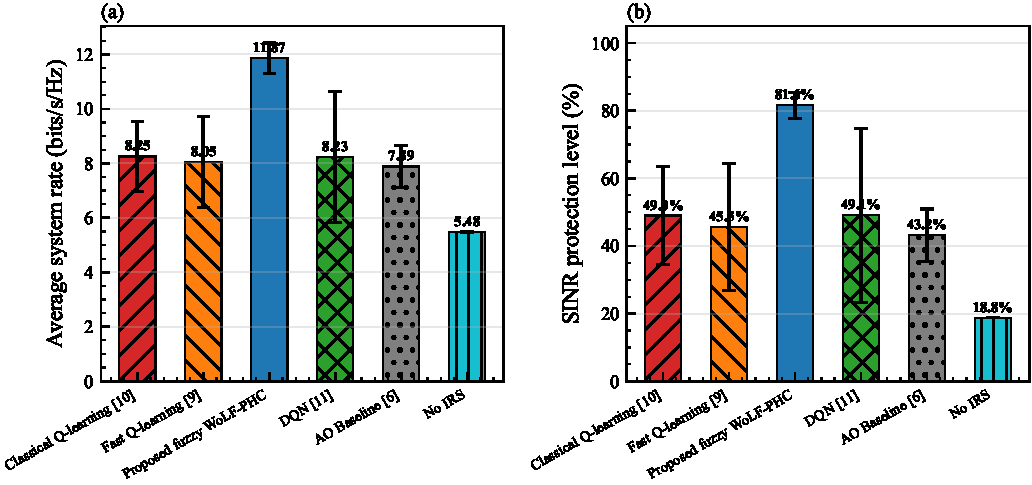
\includegraphics[width=\columnwidth]{ieee_fig9_evaluation.pdf}
\caption{Evaluation comparison: (a)~system rate and (b)~SINR protection (mean $\pm$ std, 5 seeds). Fuzzy WoLF-PHC (blue) achieves the highest performance with the smallest variance across both metrics.}
\label{fig:eval_bar}
\end{figure}

\subsection{Effect of Maximum Transmit Power}

Fig.~\ref{fig:pmax} shows rate/protection versus $P_{\max}\in\{25,32,40\}\,\text{dBm}$. WoLF-PHC rises from $1.72$ to $11.87\,\text{bits/s/Hz}$ and from $0\%$ to $81.6\%$, showing stronger scaling with available power than deterministic AO.

\begin{figure}[!t]
\centering
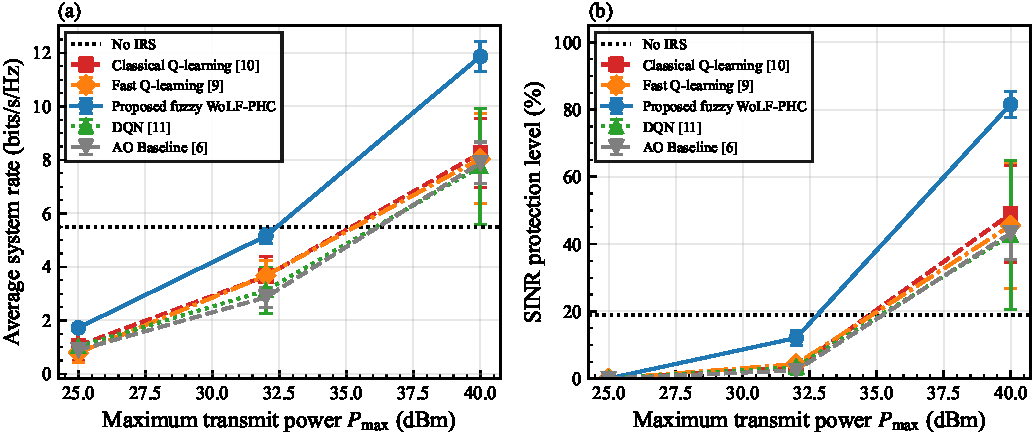
\includegraphics[width=\columnwidth]{ieee_fig5_vs_pmax.pdf}
\caption{(a)~System rate and (b)~SINR protection vs.\ maximum transmit power $P_{\max}$. WoLF-PHC scales most effectively with power, opening a gap over deterministic and tabular RL baselines at $40\,\text{dBm}$.}
\label{fig:pmax}
\end{figure}

\subsection{Effect of IRS Array Size}

Fig.~\ref{fig:nris} studies $N_\mathrm{IRS}\in\{16,64,144,256\}$. WoLF-PHC improves from $11.47$ to $11.87\,\text{bits/s/Hz}$ and from $79.2\%$ to $81.6\%$, confirming consistent gains with larger IRS size, with expected saturation at high element counts.

\begin{figure}[!t]
\centering
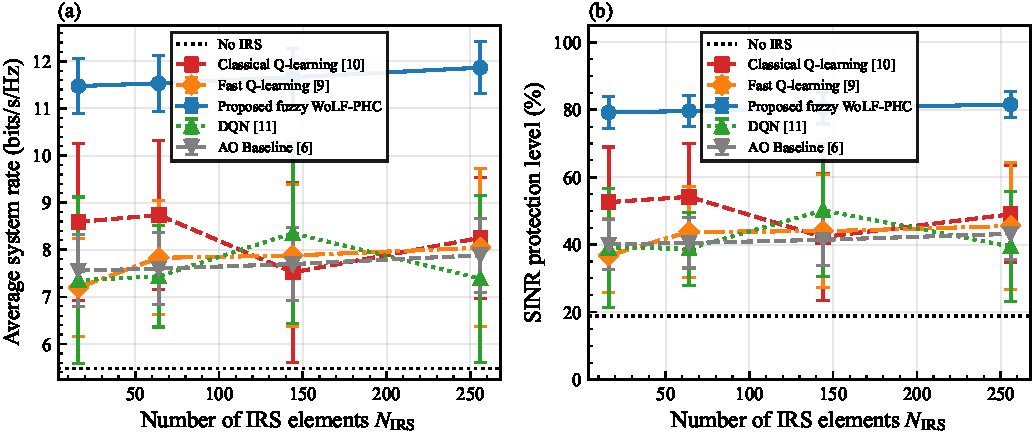
\includegraphics[width=\columnwidth]{ieee_fig6_vs_nris.pdf}
\caption{(a)~System rate and (b)~SINR protection vs.\ IRS array size $N_\mathrm{IRS}$. Performance grows with array size but saturates near $N_\mathrm{IRS}=256$; WoLF-PHC retains a consistent advantage at all scales.}
\label{fig:nris}
\end{figure}

\subsection{Effect of SINR Threshold}

Fig.~\ref{fig:sinr} evaluates $\gamma_{\min}\in\{3,5,10,15,20\}\,\text{dB}$. WoLF-PHC maintains the best trade-off across thresholds: $91.8\%$ protection at $3$~dB, $81.6\%$ at $5$~dB, and $31.4\%$ at $10$~dB. All methods collapse at $20$~dB, indicating a hard operating limit under the considered jammer.

\begin{figure}[!t]
\centering
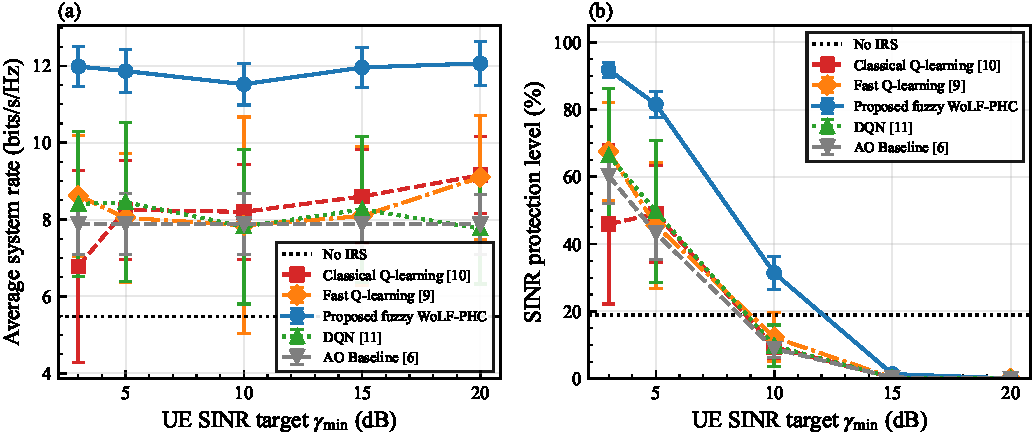
\includegraphics[width=\columnwidth]{ieee_fig7_vs_sinr.pdf}
\caption{(a)~System rate and (b)~SINR protection vs.\ UE SINR target $\gamma_{\min}$. WoLF-PHC shows the most graceful degradation with increasing SINR threshold, retaining $31.4\%$ protection at $10\,\text{dB}$.}
\label{fig:sinr}
\end{figure}

\begin{figure}[!t]
\centering
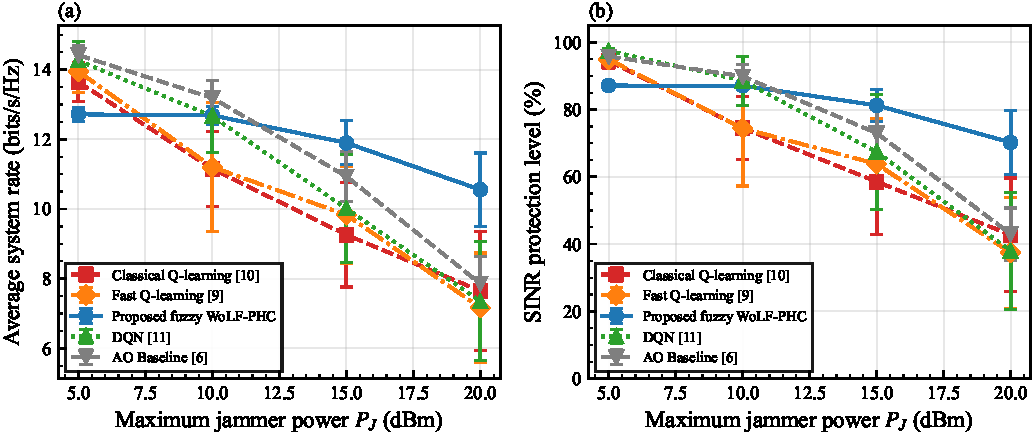
\includegraphics[width=\columnwidth]{ieee_fig12_vs_pjammer.pdf}
\caption{(a)~System rate and (b)~SINR protection vs.\ maximum jammer power $P_J$. A clear regime transition occurs near $10$--$15\,\text{dBm}$: WoLF-PHC's advantage grows with jammer power, while deterministic AO degrades sharply.}
\label{fig:pjammer}
\end{figure}


\subsection{Robustness to Jammer Power}

Fig.~\ref{fig:pjammer} shows a regime transition versus $P_J\in\{5,10,15,20\}\,\text{dBm}$. AO is competitive at low jammer power, but WoLF-PHC dominates for $P_J\geq15$~dBm and reaches $70.2\%$ protection at $20$~dBm, highlighting the value of mixed-strategy unpredictability.

\section{Conclusion}

This paper proposed a hybrid RL--AO framework for IRS-assisted anti-jamming in wideband THz systems, jointly optimizing transmit power allocation, SPDP-IRS phase control, and hybrid beamforming under adaptive jamming, with a fuzzy WoLF-PHC controller providing robust mixed-strategy power allocation. The proposed method achieves $11.87\,\text{bits/s/Hz}$ and $81.6\%$ SINR protection, outperforming the strongest baseline for each metric by $44\%$ in throughput (over Classical Q-learning) and $66\%$ in protection (over DQN) with the lowest seed variance. Parameter studies over transmit power, IRS size, SINR threshold, and jammer strength confirm consistent gains, largest in the medium/high-jamming regime where learning-based strategies dominate deterministic optimization. Future work will address imperfect CSI, multi-cell networks, and near-field THz propagation with practical IRS hardware impairments.


\balance
\begin{thebibliography}{99}
\bibitem{su2023wideband}
R.~Su, L.~Dai, and D.~W.~K.~Ng,
``Wideband precoding for RIS-aided THz communications,''
\emph{IEEE Trans.\ Commun.}, vol.~71, no.~6, pp.~3592--3604, Jun.\ 2023.

\bibitem{yan2023beamforming}
W.~Yan, W.~Hao, C.~Huang, G.~Sun, O.~Muta, H.~Gacanin, and C.~Yuen,
``Beamforming analysis and design for wideband THz reconfigurable intelligent surface communications,''
\emph{IEEE J.\ Sel.\ Areas Commun.}, vol.~41, no.~8, pp.~2306--2320, Aug.\ 2023.

\bibitem{hanawal2016joint}
M.~K.~Hanawal, M.~J.~Abdel-Rahman, and M.~Krunz,
``Joint adaptation of frequency hopping and transmission rate for anti-jamming wireless systems,''
\emph{IEEE Trans.\ Mobile Comput.}, vol.~15, no.~9, pp.~2247--2259, Sep.\ 2016.

\bibitem{xu2018jamming}
Y.~Xu, G.~Ren, J.~Chen, Y.~Luo, and L.~Jia,
``Anti-jamming transmission in cognitive radio networks with unknown channel statistics,''
\emph{IEEE Trans.\ Wireless Commun.}, vol.~17, no.~2, pp.~765--779, Feb.\ 2018.

\bibitem{akyildiz2022thz}
I.~F.~Akyildiz, J.~M.~Jornet, and C.~Han,
``Terahertz band: Next frontier for wireless communications,''
\emph{Physical Communication}, vol.~12, pp.~16--32, Sep.\ 2014.

\bibitem{wu2019intelligent}
Q.~Wu and R.~Zhang,
``Intelligent reflecting surface enhanced wireless network via joint active and passive beamforming,''
\emph{IEEE Trans.\ Wireless Commun.}, vol.~18, no.~11, pp.~5394--5409, Nov.\ 2019.

\bibitem{wu2021irs_survey}
Q.~Wu, S.~Zhang, B.~Zheng, C.~You, and R.~Zhang,
``Intelligent reflecting surface-aided wireless communications: A tutorial,''
\emph{IEEE Trans.\ Commun.}, vol.~69, no.~5, pp.~3313--3351, May 2021.

\bibitem{renzo2020smart}
M.~Di~Renzo \emph{et al.},
``Smart radio environments empowered by reconfigurable intelligent surfaces: How it works, state of research, and the road ahead,''
\emph{IEEE J.\ Sel.\ Areas Commun.}, vol.~38, no.~11, pp.~2450--2525, Nov.\ 2020.

\bibitem{yang2021irs}
H.~Yang, Z.~Xiong, J.~Zhao, D.~Niyato, Q.~Wu, H.~V.~Poor, and M.~Tornatore,
``Intelligent reflecting surface assisted anti-jamming communications: A fast reinforcement learning approach,''
\emph{IEEE Trans.\ Wireless Commun.}, vol.~20, no.~3, pp.~1963--1976, Mar.\ 2021.

\bibitem{watkins1992q}
C.~J.~C.~H.~Watkins and P.~Dayan,
``Q-learning,''
\emph{Machine Learning}, vol.~8, no.~3--4, pp.~279--292, 1992.

\bibitem{mnih2015human}
V.~Mnih \emph{et al.},
``Human-level control through deep reinforcement learning,''
\emph{Nature}, vol.~518, no.~7540, pp.~529--533, Feb.\ 2015.

\bibitem{bowling2002wolf}
M.~Bowling and M.~Veloso,
``Multiagent learning using a variable learning rate,''
\emph{Artif.\ Intell.}, vol.~136, no.~2, pp.~215--250, 2002.

\end{thebibliography}

\end{document}
